\documentclass{article}%
\usepackage[T1]{fontenc}%
\usepackage[utf8]{inputenc}%
\usepackage{lmodern}%
\usepackage{textcomp}%
\usepackage{lastpage}%
\usepackage[head=40pt,margin=0.5in,bottom=0.6in]{geometry}%
\usepackage{graphicx}%
%
\title{\textbf{Trabajadores de Conferry exigieron la recuperación de las embarcaciones}}%
\author{EL NACIONAL WEB}%
\date{21/09/2018}%
%
\begin{document}%
\normalsize%
\maketitle%
\textbf{URL: }%
http://www.el{-}nacional.com/noticias/protestas/trabajadores{-}conferry{-}exigieron{-}recuperacion{-}las{-}embarcaciones\_252675\newline%
%
\textbf{Periodico: }%
EN, %
ID: %
252675, %
Seccion: %
Protestas\newline%
%
\textbf{Palabras Claves: }%
Protestas, Denuncia\newline%
%
\textbf{Derecho: }%
2.3, %
Otros Derechos: %
, %
Sub Derechos: %
2.3.4\newline%
%
\textbf{EP: }%
SI\newline%
\newline%
%
\textbf{\textit{Los empleados manifestaron por segundo día consecutivo para exigir el pago del sueldo actual}}%
\newline%
\newline%
%
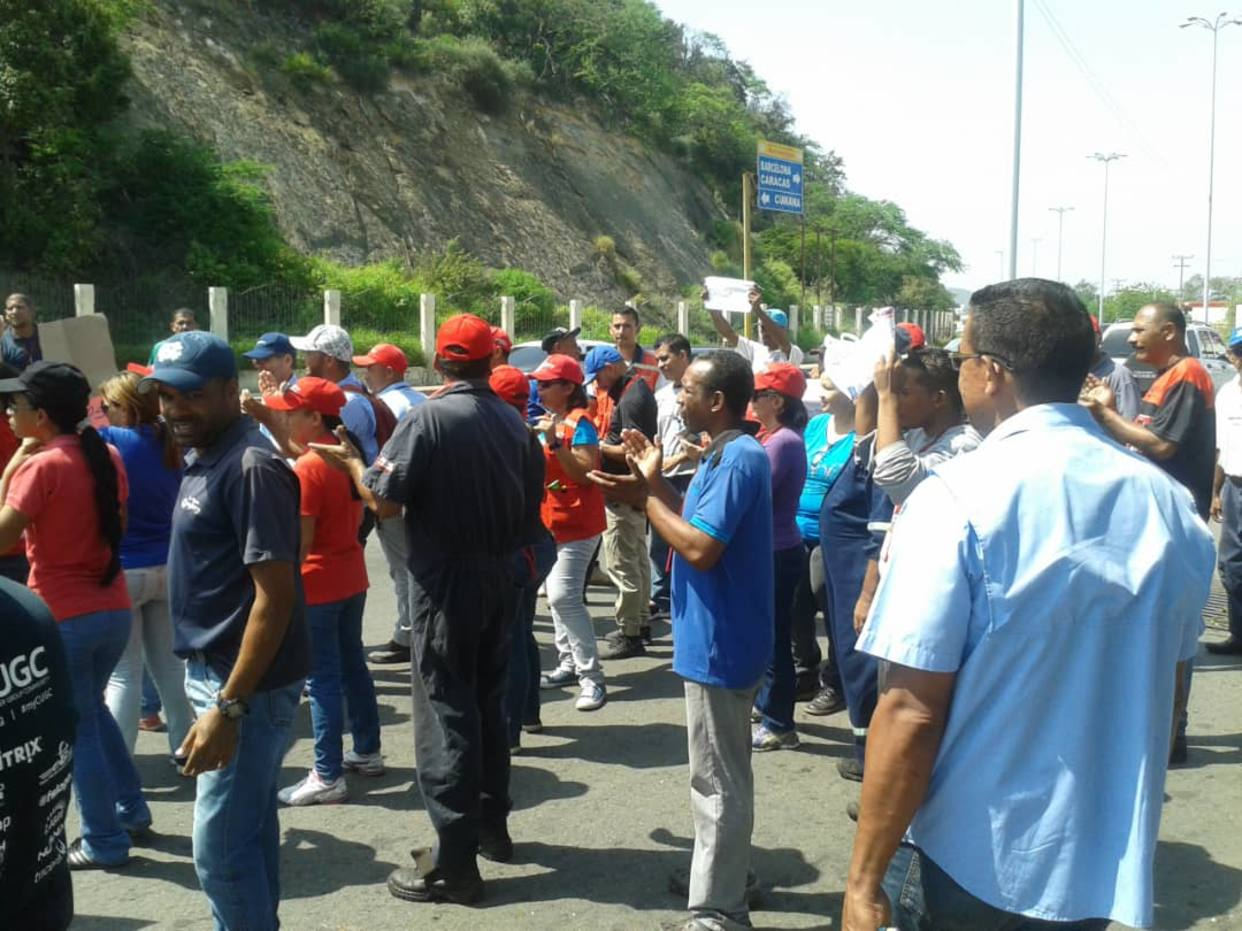
\includegraphics[width=300px]{241.jpg}%
\newline%
%
Trabajadores de la empresa de navíos~Conferry protestaron~este viernes, para exigir la cancelación del salario y~la recuperación de las embarcaciones que están paralizadas.%
\newline%
%
"Los trabajadores estamos pidiendo la recuperación de la empresa,~estamos capacitados para sacarla adelante. Solo hace falta voluntad del Estado para unificar a los trabajadores", indicó uno de los voceros de la empresa.%
\newline%
%
Los manifestantes protestaron~en el terminal marítimo en señal de protesta por segundo día consecutivo, para exigir el pago correcto del sueldo actual luego del incremento salarial.%
\newline%
%
\end{document}